\documentclass[twocolumn]{article}
\usepackage[margin=1in]{geometry}
\usepackage{graphicx}
\graphicspath{ {C:/John/LaTeX/Scioly/Protein/main/images/} }
\usepackage{grffile}

\title{Protein Modeling Event Guide}
\author{John Yang}
\date{March 22, 2019}

\begin{document}

\twocolumn[
\begin{@twocolumnfalse}
\maketitle
\begin{abstract}
The protein modeling event will most likely return for the 2020 season. The event consists of three parts: 1) A prebuild model 2) an onsite model and 3) A written test. The focus topic of each year will change, but the principles are the same and protein biology and biochemistry aspects will usually remain the same. Here, we will go over strategies for each of the three portions of the event, and some helpful resources to use. 
\end{abstract}
\end{@twocolumnfalse}
]

\section{Prebuild Models}
Each year, a new topic will be selected. For 2019, the topic was CRISPR Cas9/Anti-CRISPR. In the rules, it will tell you which residues you will have to model. These residues will be selected from a main PDB file that will be the same for the whole year. 
\subsection{Using Jmol}
On the MSOE website, there will be a link to an online version of Jmol (Link below). However, I also highly reccomend downloading an offline version to give you more flexibility. Links are provided in the resources section. I will discuss the offline version here, especially since it requires a few more steps. \\
After starting Jmol, you will get a window with a black screen. Click `open' under File, and select the file you want. From there, you will have to open the console (Fig. 1). 
\begin{figure}[h]
\caption{Opening the console}
\centering
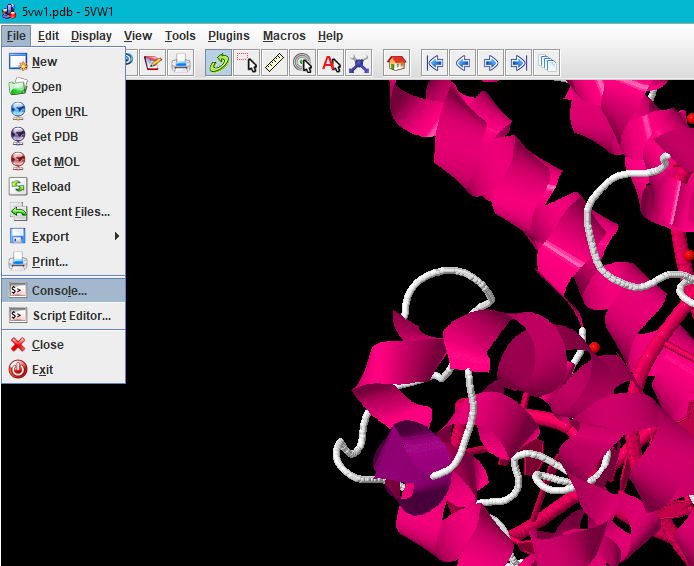
\includegraphics[scale=0.4]{console}
\end{figure}
From there, you will get a window, shown in Fig. 2. 
\begin{figure}[h]
\caption{The console}
\centering
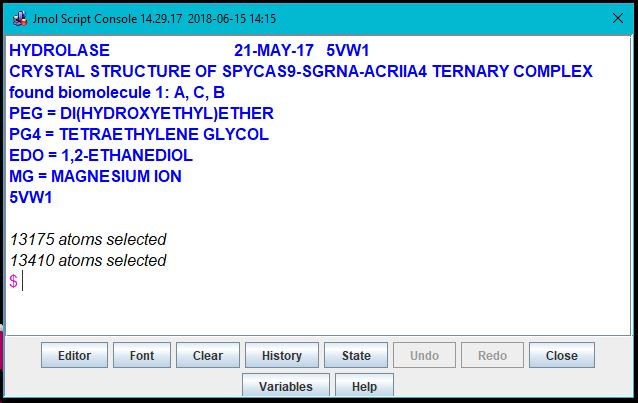
\includegraphics[scale=0.45]{console-1}
\end{figure}
From here, you can type in any commands you need. A Jmol reference sheet has been included. It also contains a chart of the 20 amino acids. In general, the most important commands are 
{\fontfamily{qcr}\selectfont restrict}, {\fontfamily{qcr}\selectfont select}, {\fontfamily{qcr}\selectfont color}, and {\fontfamily{qcr}\selectfont backbone 1.5}. 

To learn how to fold a model, go to the Onsite Build section (Section 2). It is mostly the same, but without the required sidechains. 
\subsection{Creative Additions}
Which additions you use will depend on the protein you are modeling. Good ideas include substrates, important sidechains (i.e. active sites), Parts of other proteins it interacts with, etc. Make sure you can explain why those additions are important. On your index card, you will have to make a chart regarding this. I will provide past index cards, and the format is on the MSOE website. When adding sidechains, don't add every single one in the protein (You will lose points). Instead, find out which ones are the most important and add those. You also aren't limited to the sidechains from MSOE. You can use any material you want as long as you notate it on your index cards. 
\subsection{Mounting Your Protein}
Doing this well will make your protein visually appealing and easy for the judges to grade. We tried two methods this year. The first was a suspension model, where we made a frame out of dowels, and tied fishing line to the protein to make it seem as if it was floating in midair. (Fig. 3)
\begin{figure}[h!]
\caption{A suspension model}
\centering
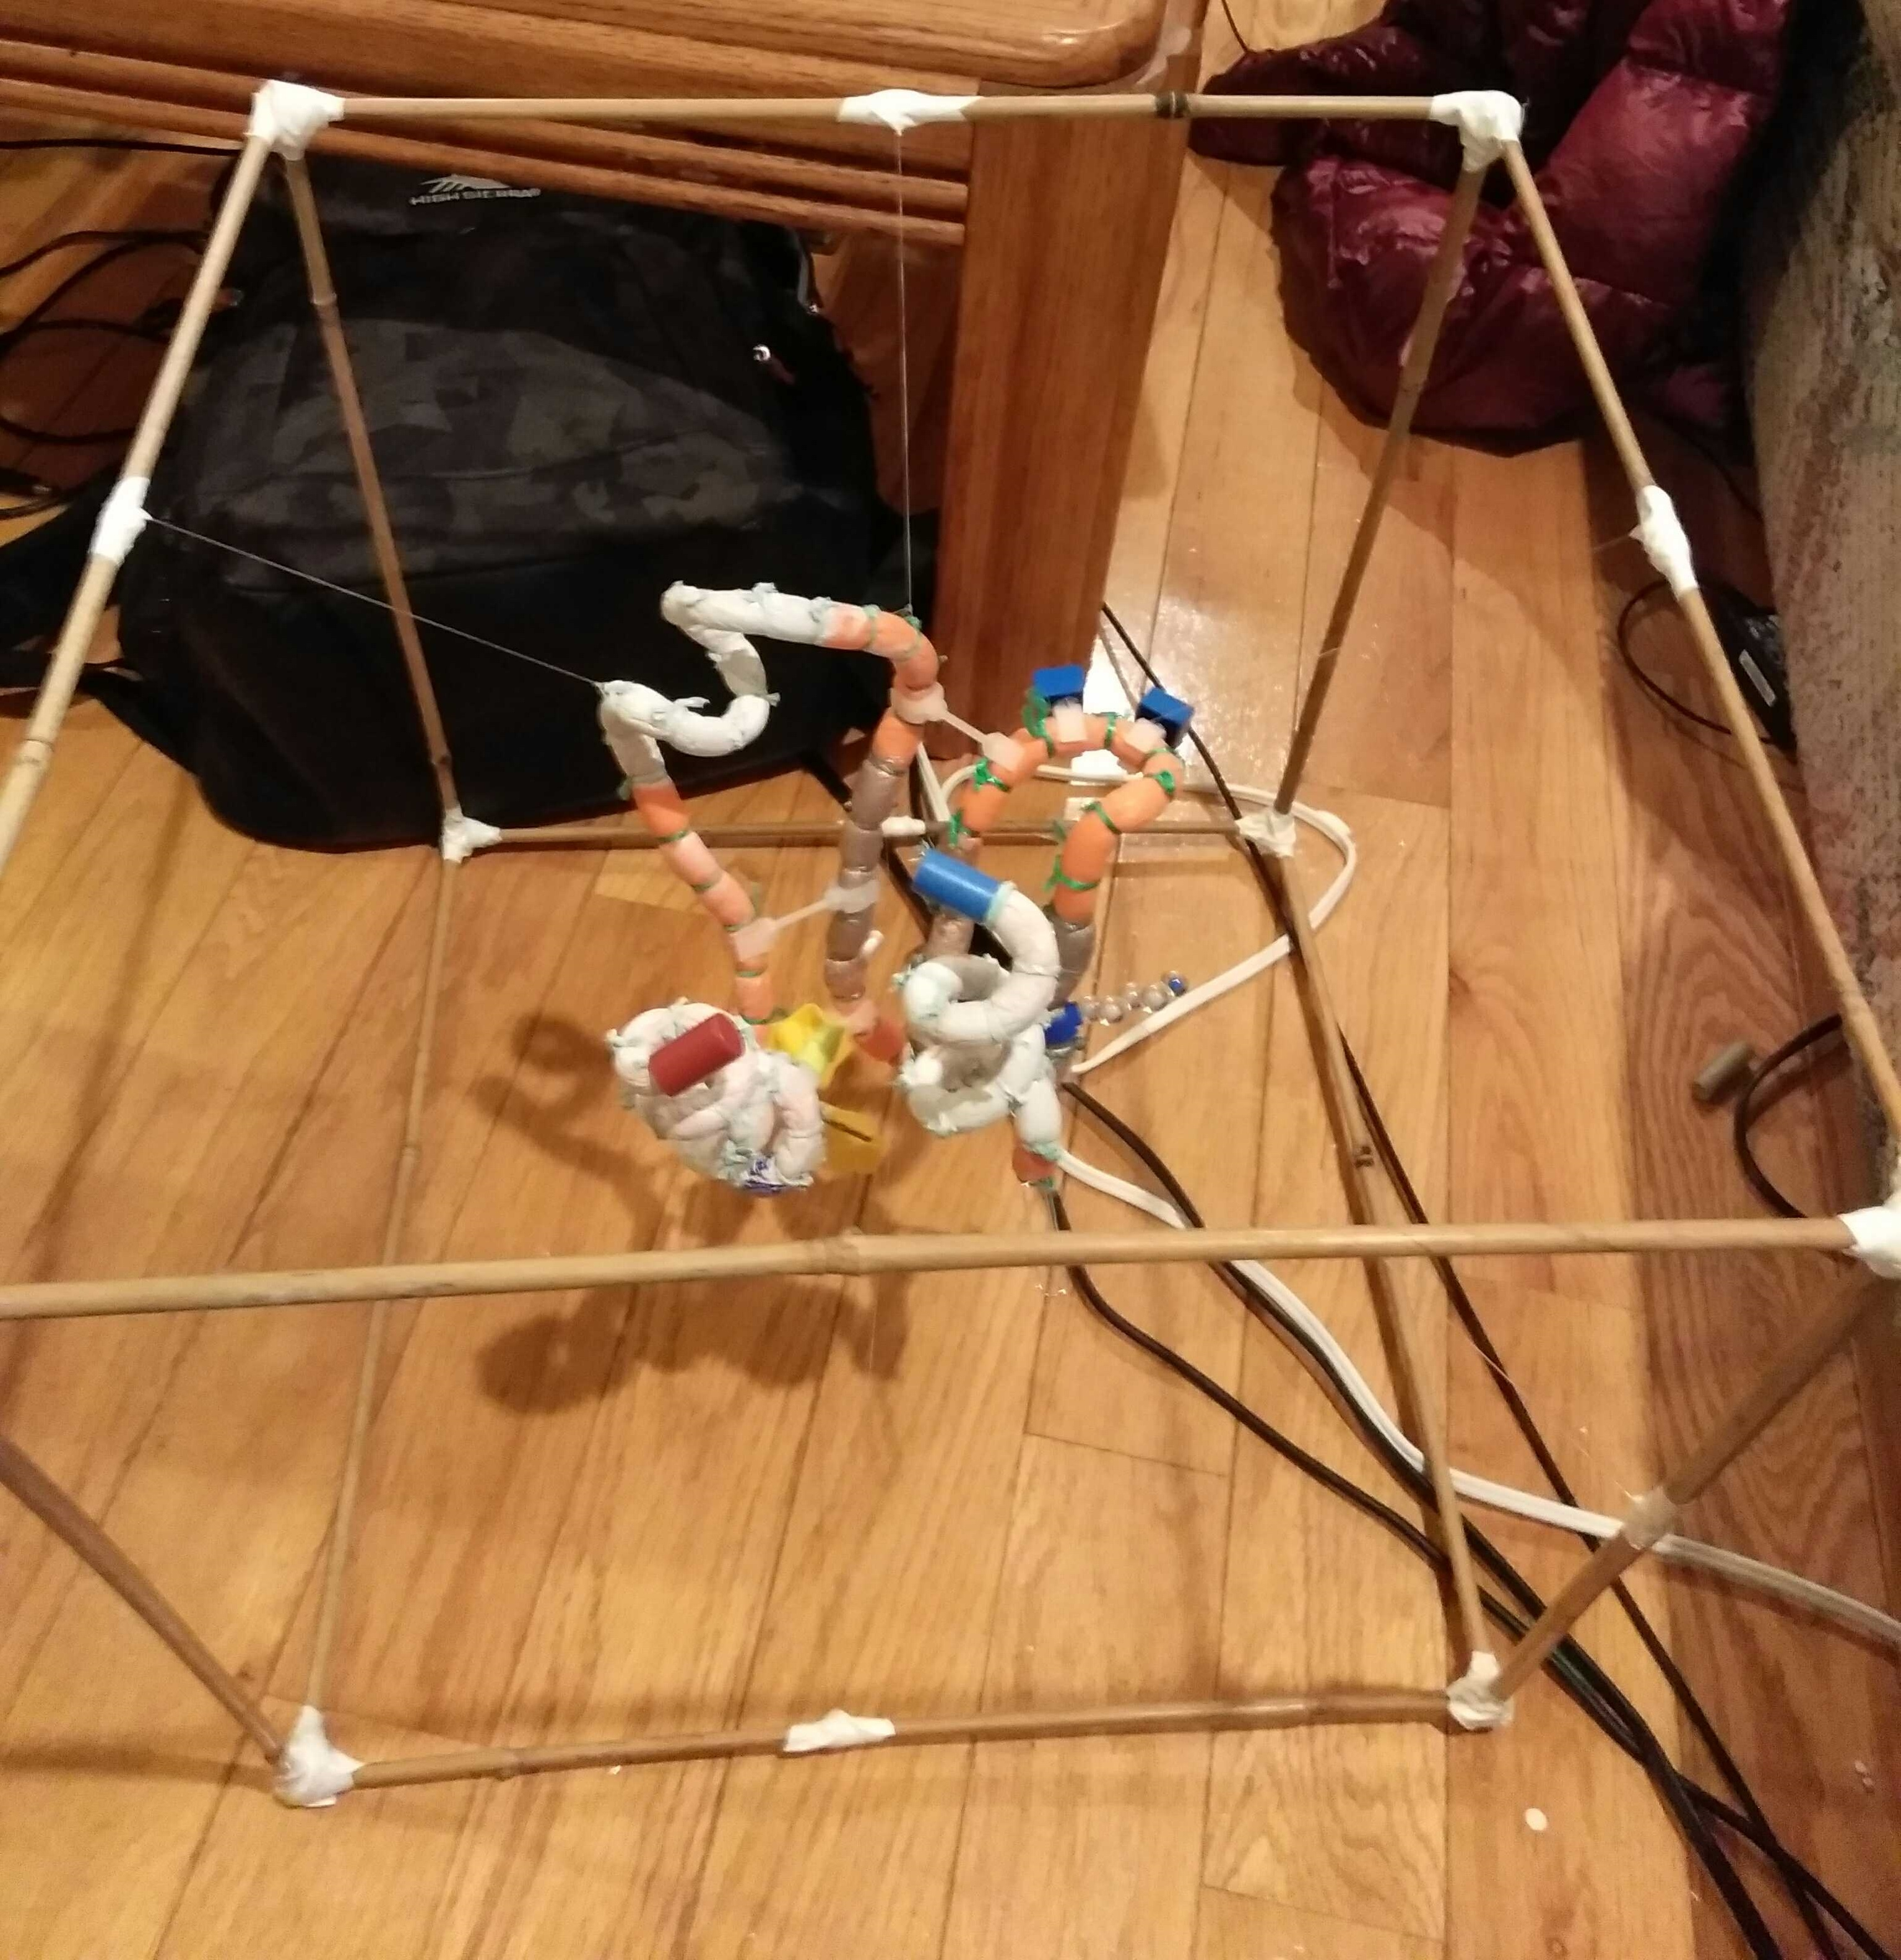
\includegraphics[scale=0.09]{suspension}
\end{figure}
The second was a model where dowels were used to support the various different sidechains. This was a lot easier to build, but ended up looking more cluttered. This approach was the one we ended up using at states. (Fig. 4)
\begin{figure}[h!]
\caption{Our final states model}
\centering
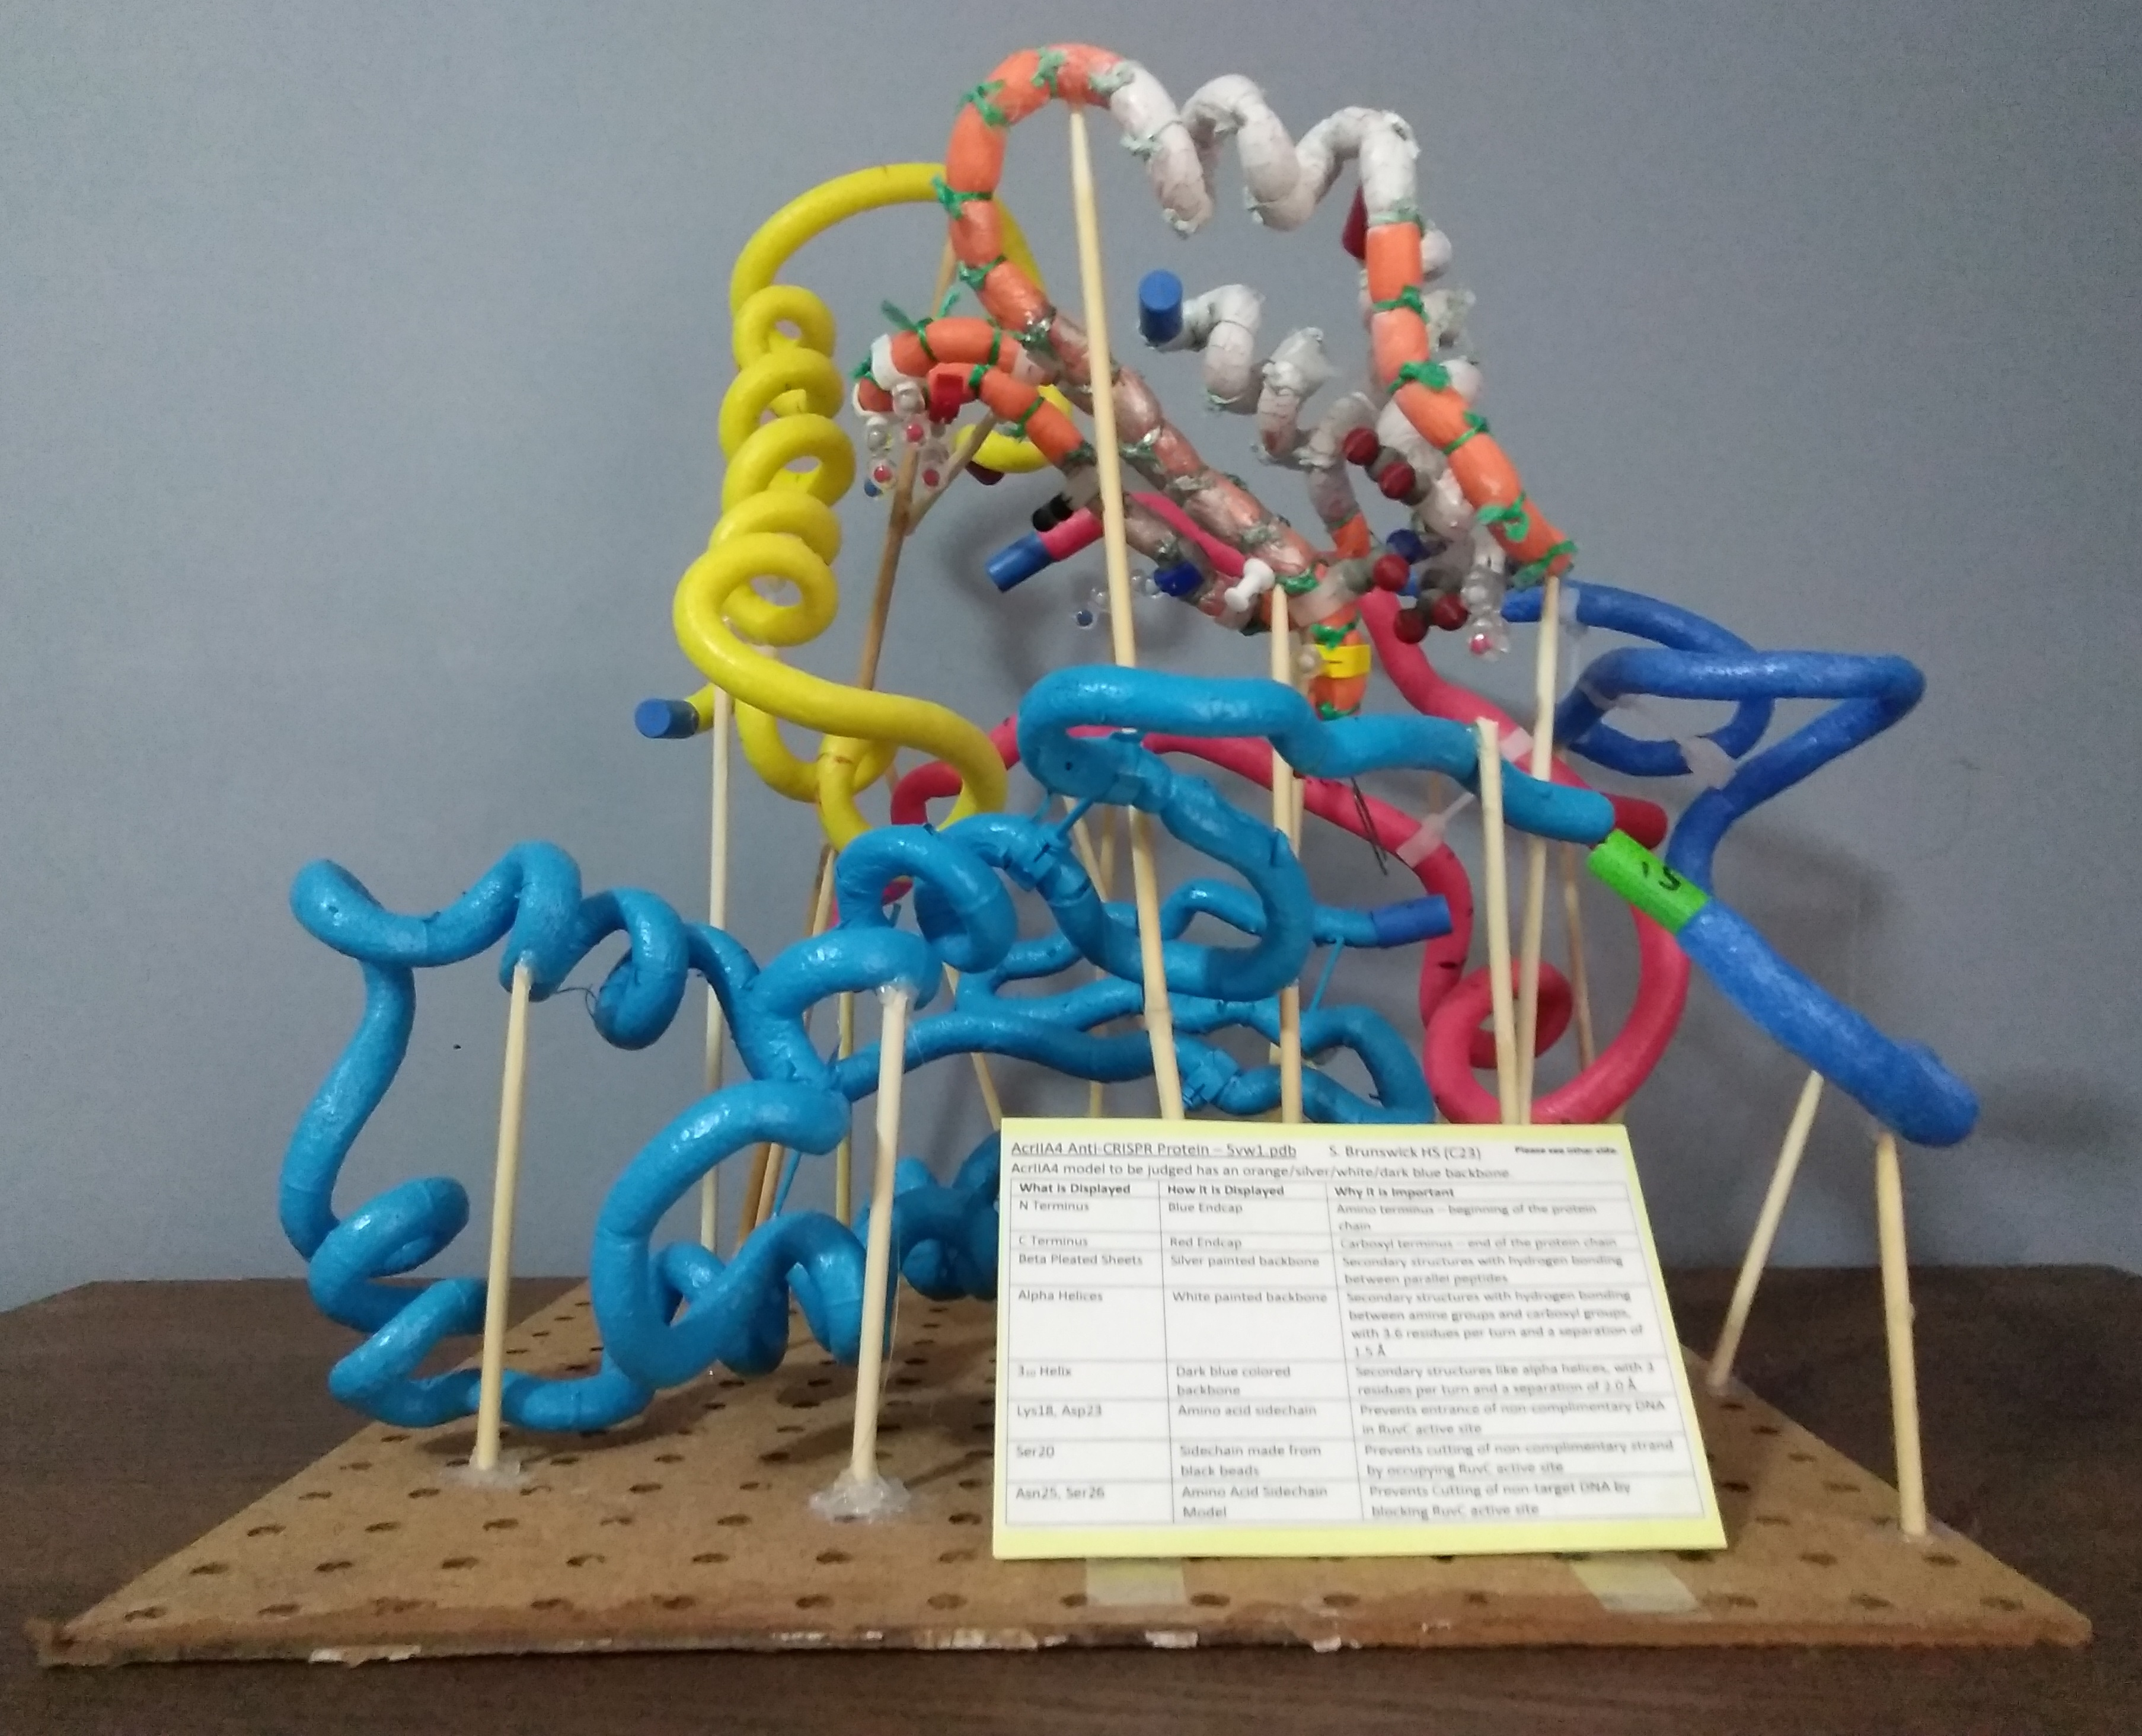
\includegraphics[scale=0.06]{states}
\end{figure}

With anything, remember that accuracy is the priority. Don't use a mounting method that will mess up the actual structure of the protein. 

Another thing with prebuilds is that you can make it more visually appealing than an onsite build. I reccomend using spray paint to differentiate between different secondary structures. You can also use zip ties or string to mark the residues. 
\section{On-Site Build}
\subsection{Folding a model}
Here, we will fold residues 718-764 or chain B from 5f9r.pdb. The key sidechains are Asp745 and Leu738. (Fig. 5)
\begin{figure}[h!]
\caption{A sample onsite build}
\centering
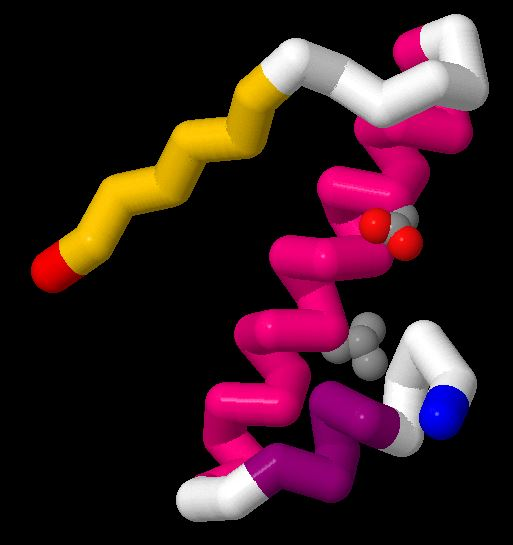
\includegraphics[scale=0.5]{onsite}
\end{figure}

First, make sure you have all the materials you need. You will need a ruler, sharpie, mini-toober, sidechains, endcaps, and support posts. (Fig. 6)
\begin{figure}[h!]
\caption{Required materials}
\centering
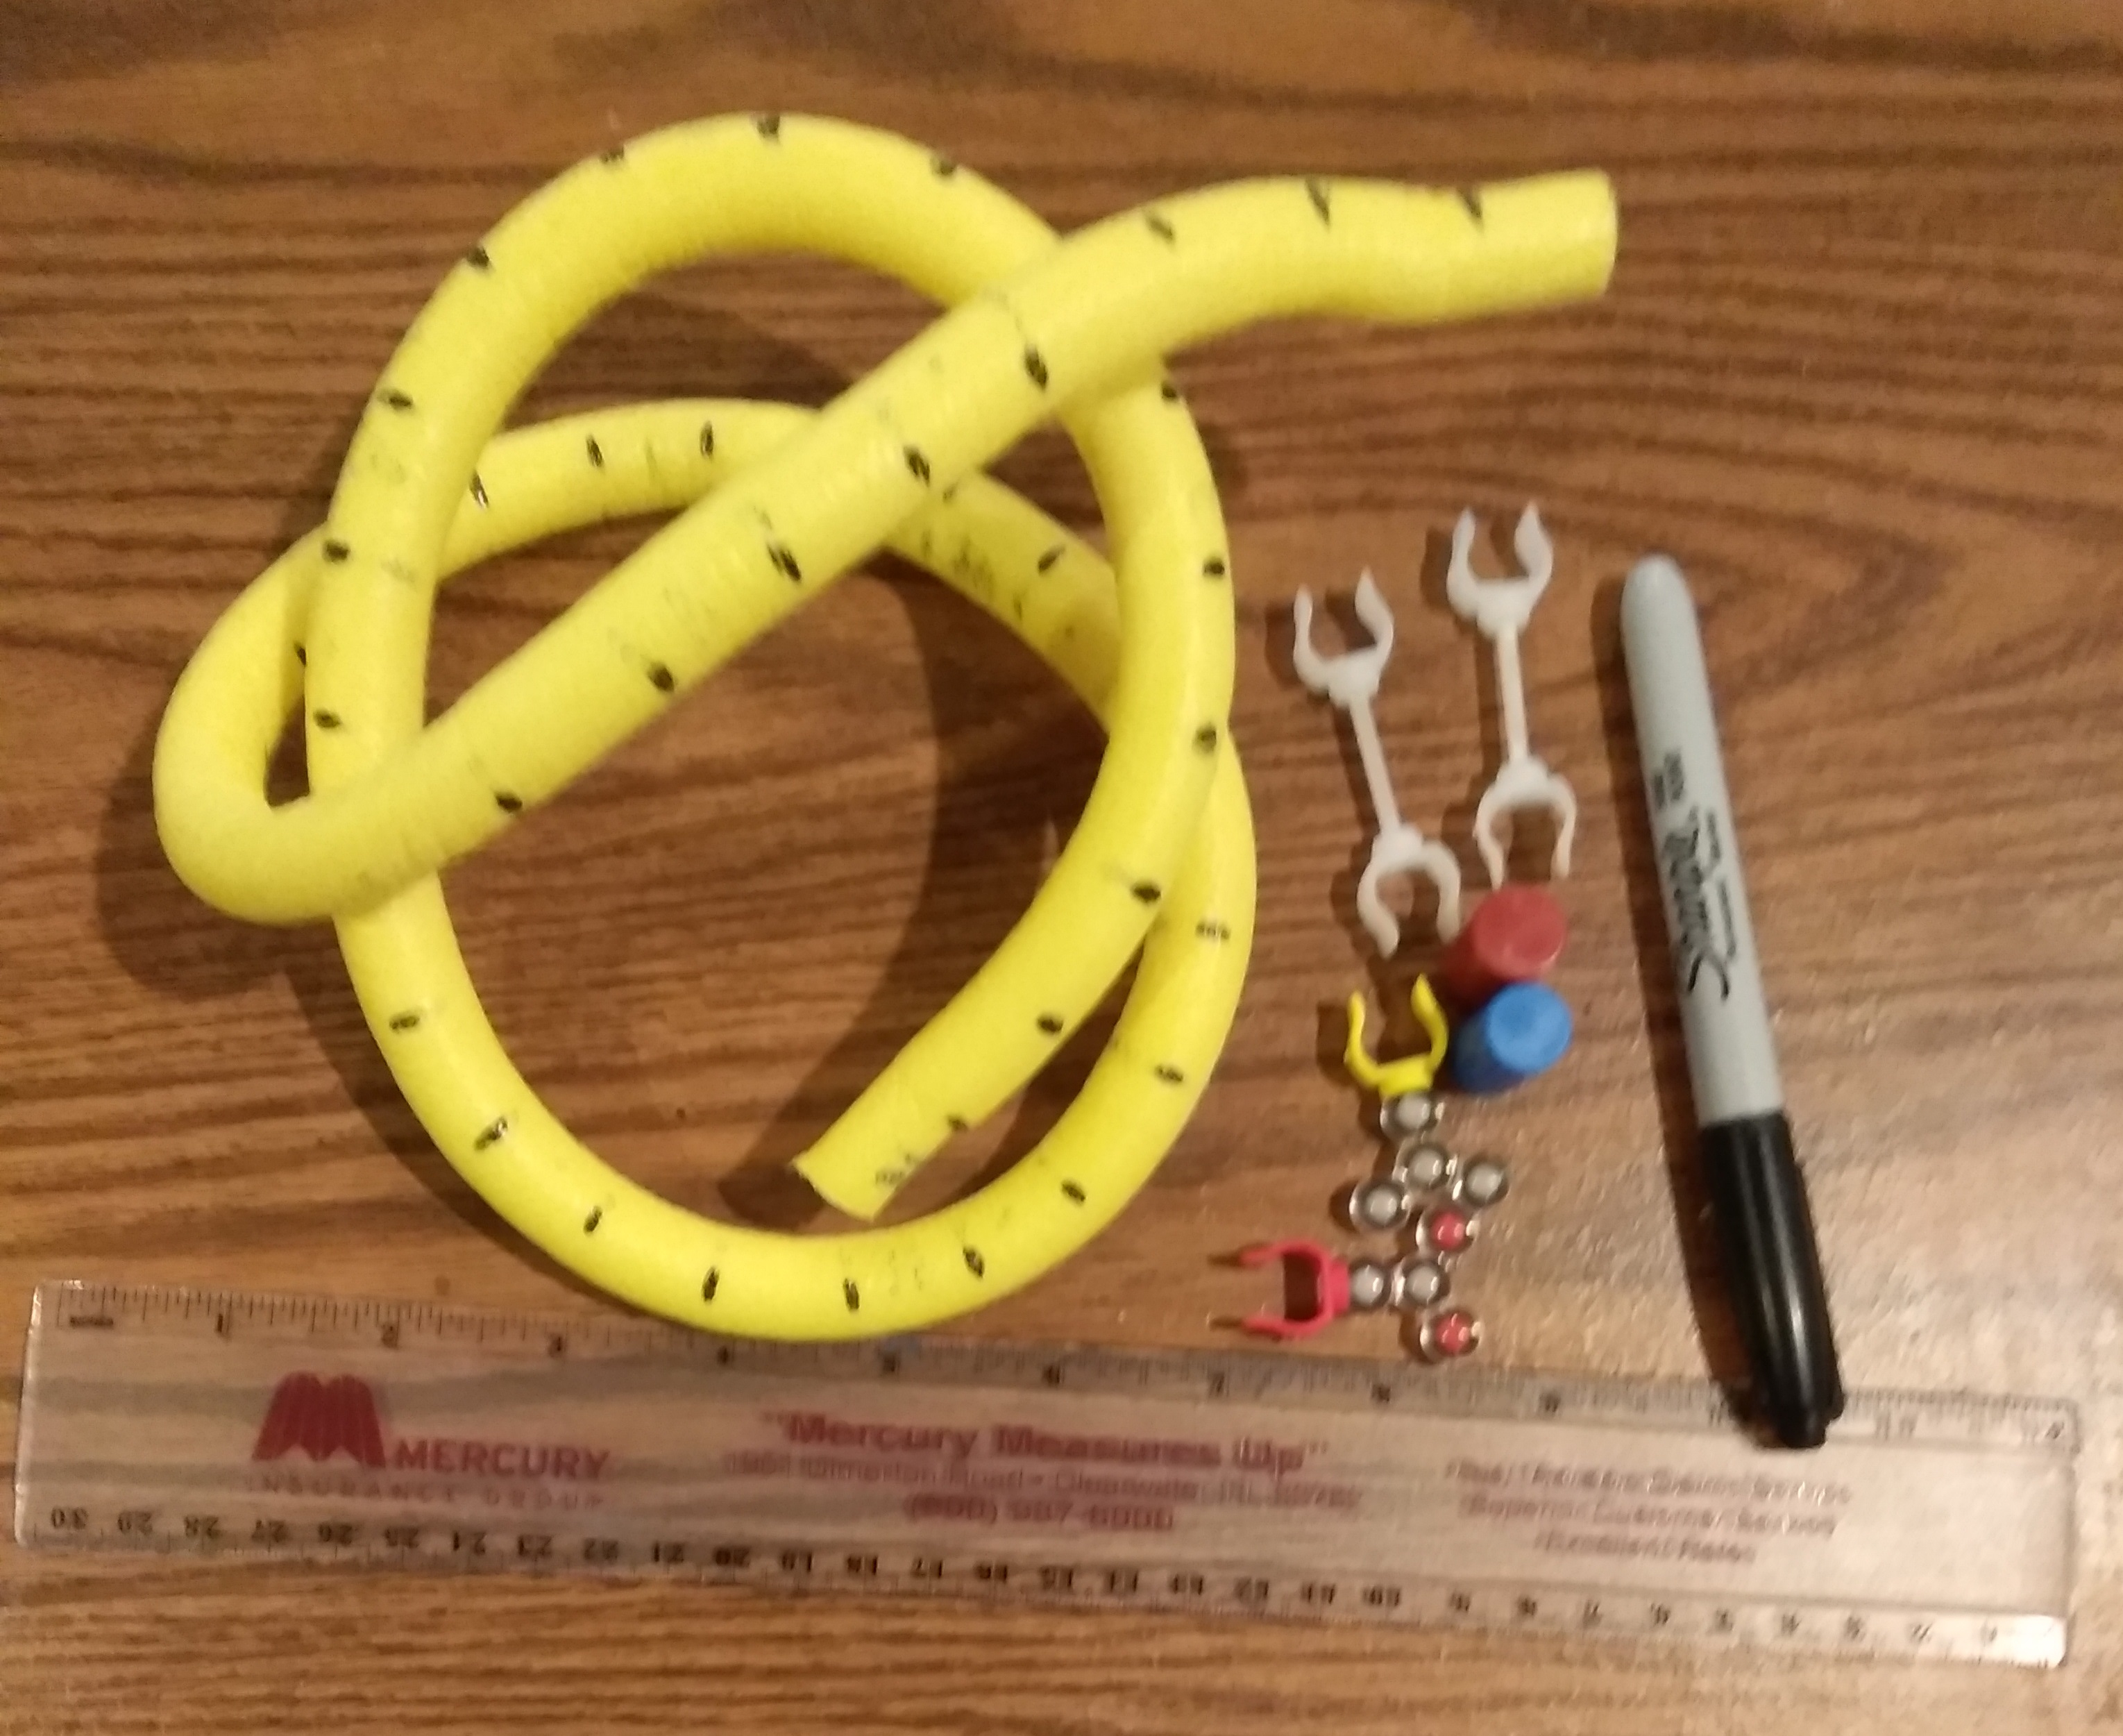
\includegraphics[scale=0.07]{materials}
\end{figure}
The first thing you should do is type in your Jmol commands until you get what you need. In the beginning, when you practice, you can use the Jmol reference, but don't plan on having it at competitions. If you need to, this might be something you'd want to put on your cheatsheet. Try to only take 1-2 minutes for this part. 

From there, mark out every 2 cm, since the scale is 2 cm per amino acid. It may also be helpful to use an extra thick line on multiples of 10, so counting is easier. In general, mark anything you need, as you won't be judged by this, and it will help you. From here, using Jmol, hover your mouse over the places where it changes color (structure) and note the number residue it is. In the offline version, you can also just click on it and it will show up in the console. Mark these places using `A' for alpha helix, `B' for beta sheet, and `$3_{10}$' for a $3_{10}$ helix (or your own conventions). In Jmol, pink is alpha helix, yellow is beta sheet, and magenta is $3_{10}$ helix. Try to have the marking part only take 3-4 minutes. 

The next thing you should do is place the endcaps onto the correct ends. The lower number is always the N-terminus, and always the blue cap. After doing this step, begin to fold the secondary structures. 

For folding purposes, both types of helices are treated mostly the same. The difference is, after folding a $3_{10}$ helix, stretch it out a little more (lengthwise). To fold a helix, wrap the mini-toober around your finger from where you marked the residues. Remove your finger and twist it tighter, so that the inside circle is about the size of a barbecue skewer. In general, make sure it looks the same as the Jmol version and has the same number of turns. Make sure it is right-handed, meaning that you fold it counterclockwise. A good way to check for this is to imagine that the helix is a spiral staircase. If you would put your right hand on a railing to the outside of the stairs, then the helix is right handed. (Fig. 7) If it doesn't have enough turns, it's probably not tight enough. 
\begin{figure}[h!]
\caption{A folded helix. Notice the tightness and separation. The Jmol version has 6 turns, and so does this. }
\centering
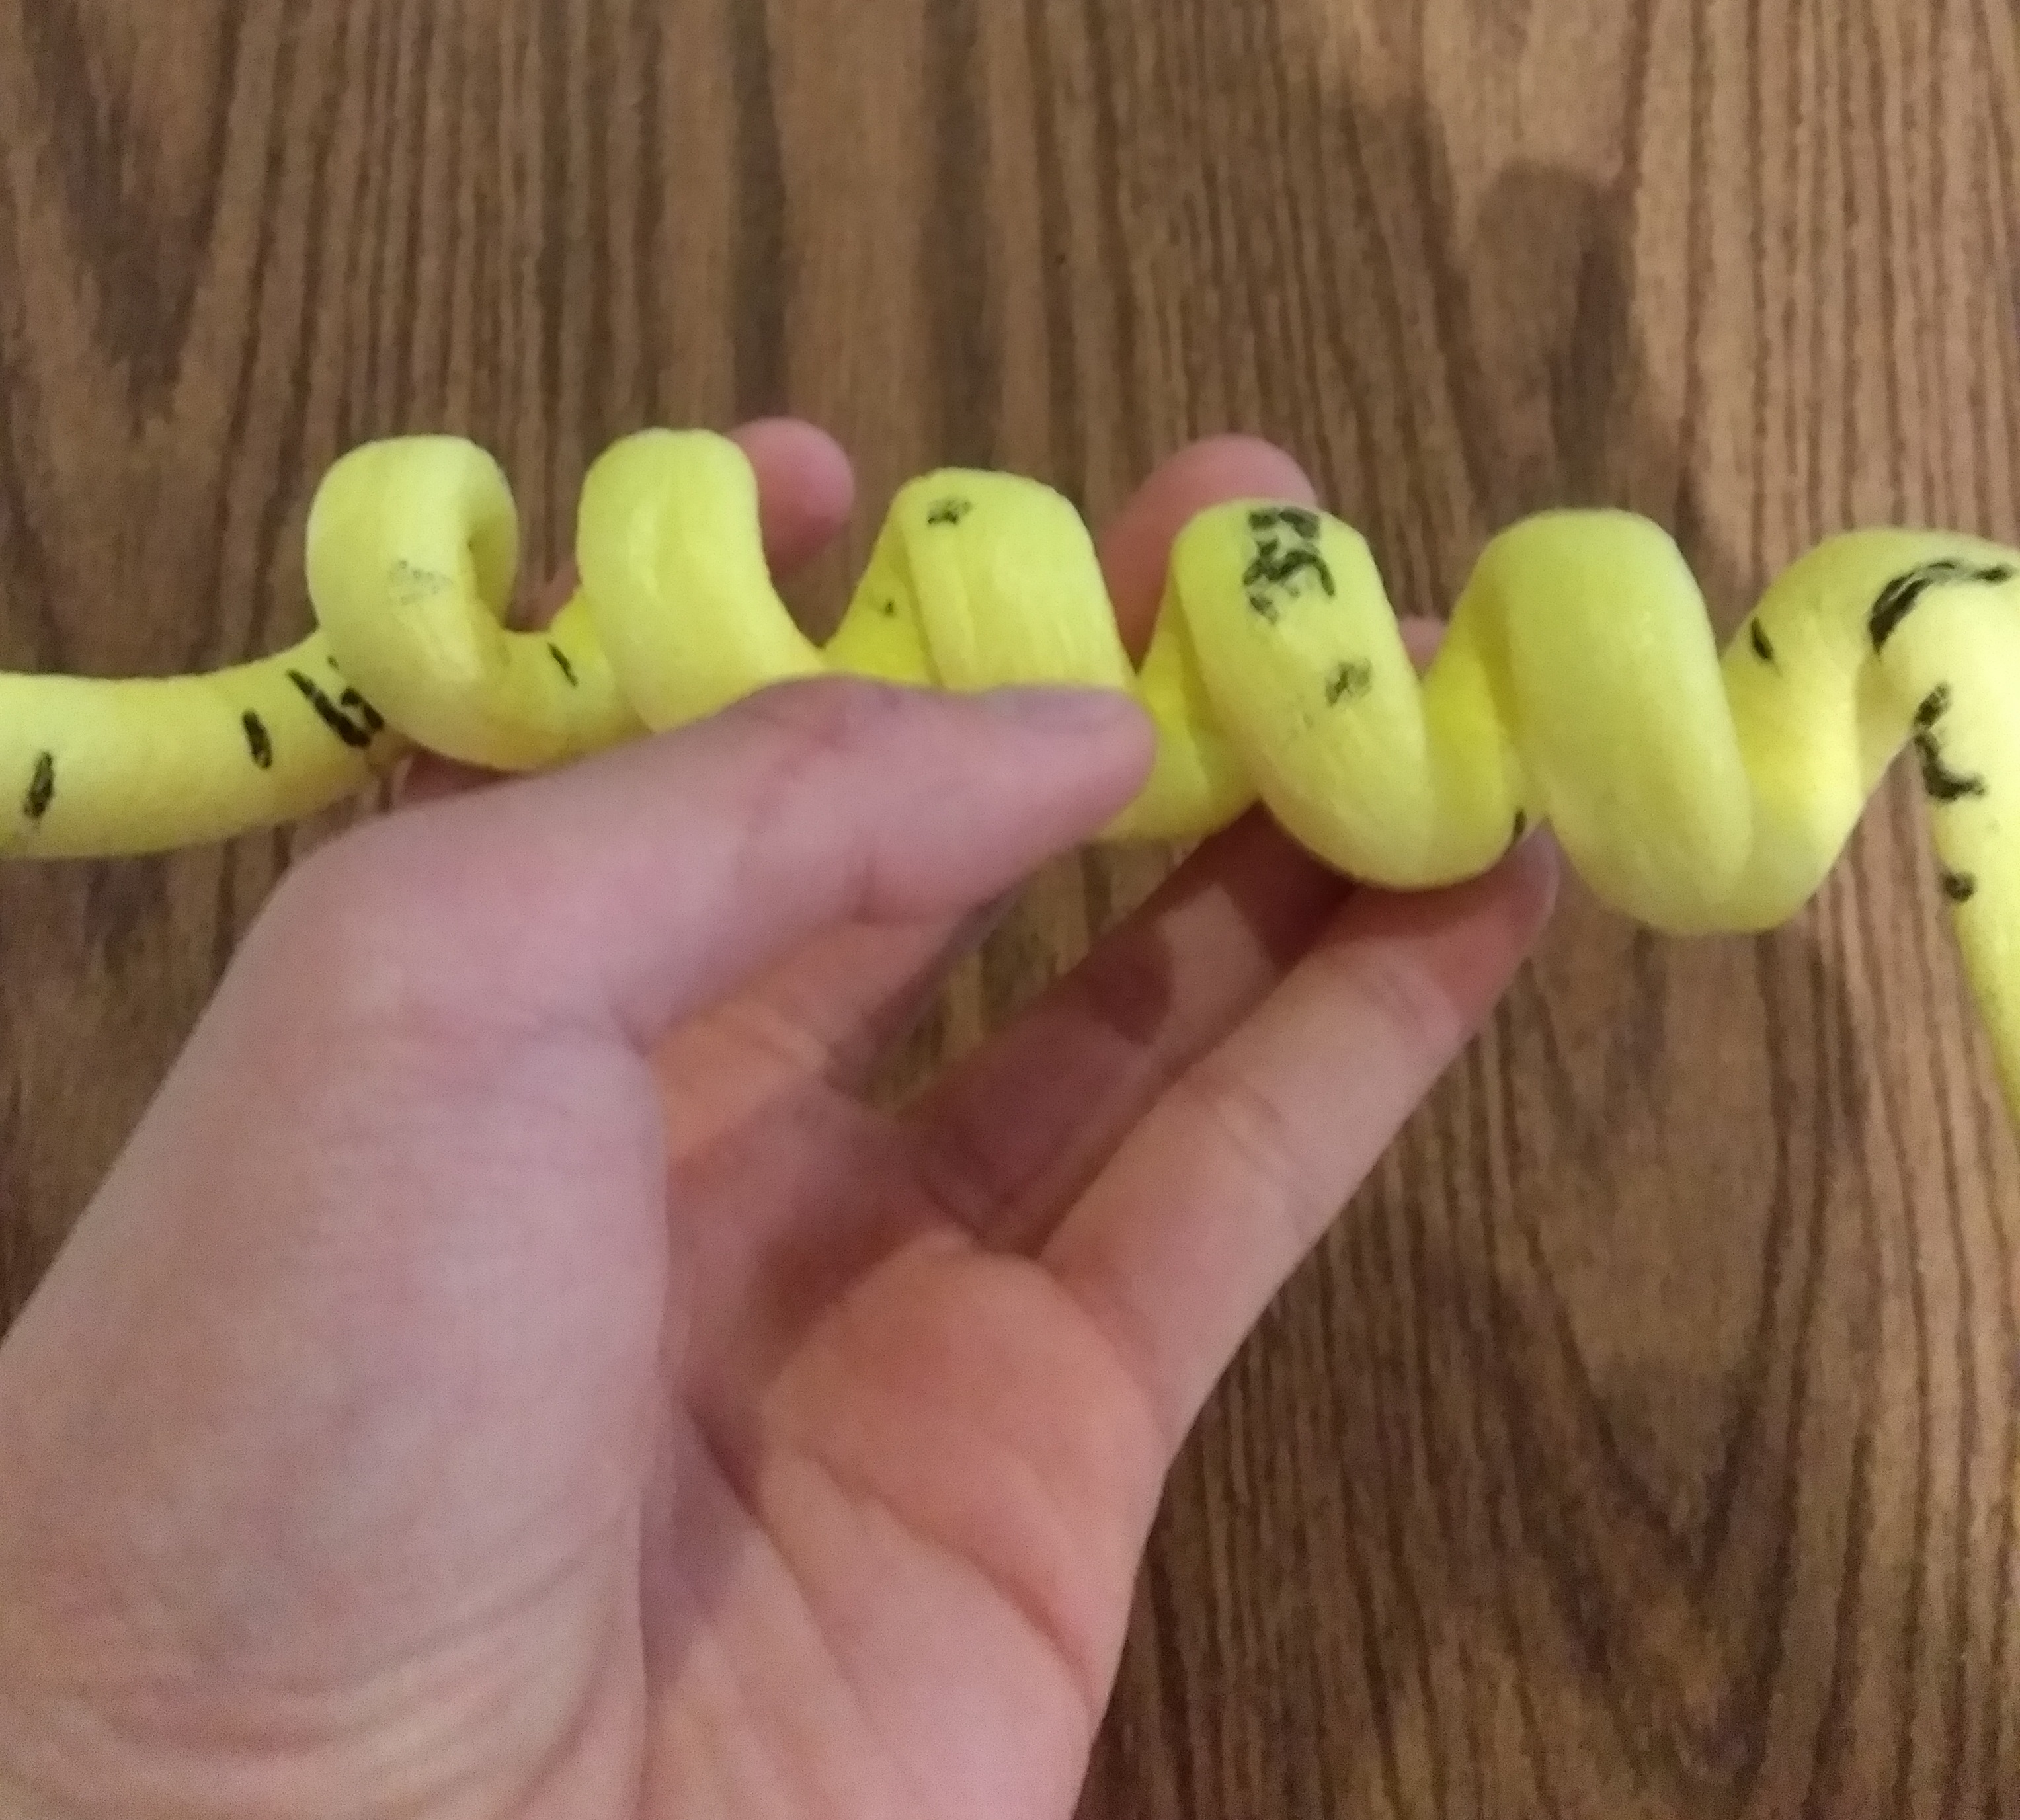
\includegraphics[scale=0.07]{helix}
\end{figure}

To fold a beta sheet, take the section of toober and kink it up and down, one for each residue. Try to make it sharp, but not too sharp. (Fig. 8) At competitions, you can also shade in the beta sheets with your marker so it's more clear. 

\begin{figure}[h!]
\caption{A beta sheet. Notice how it is kinked. }
\centering
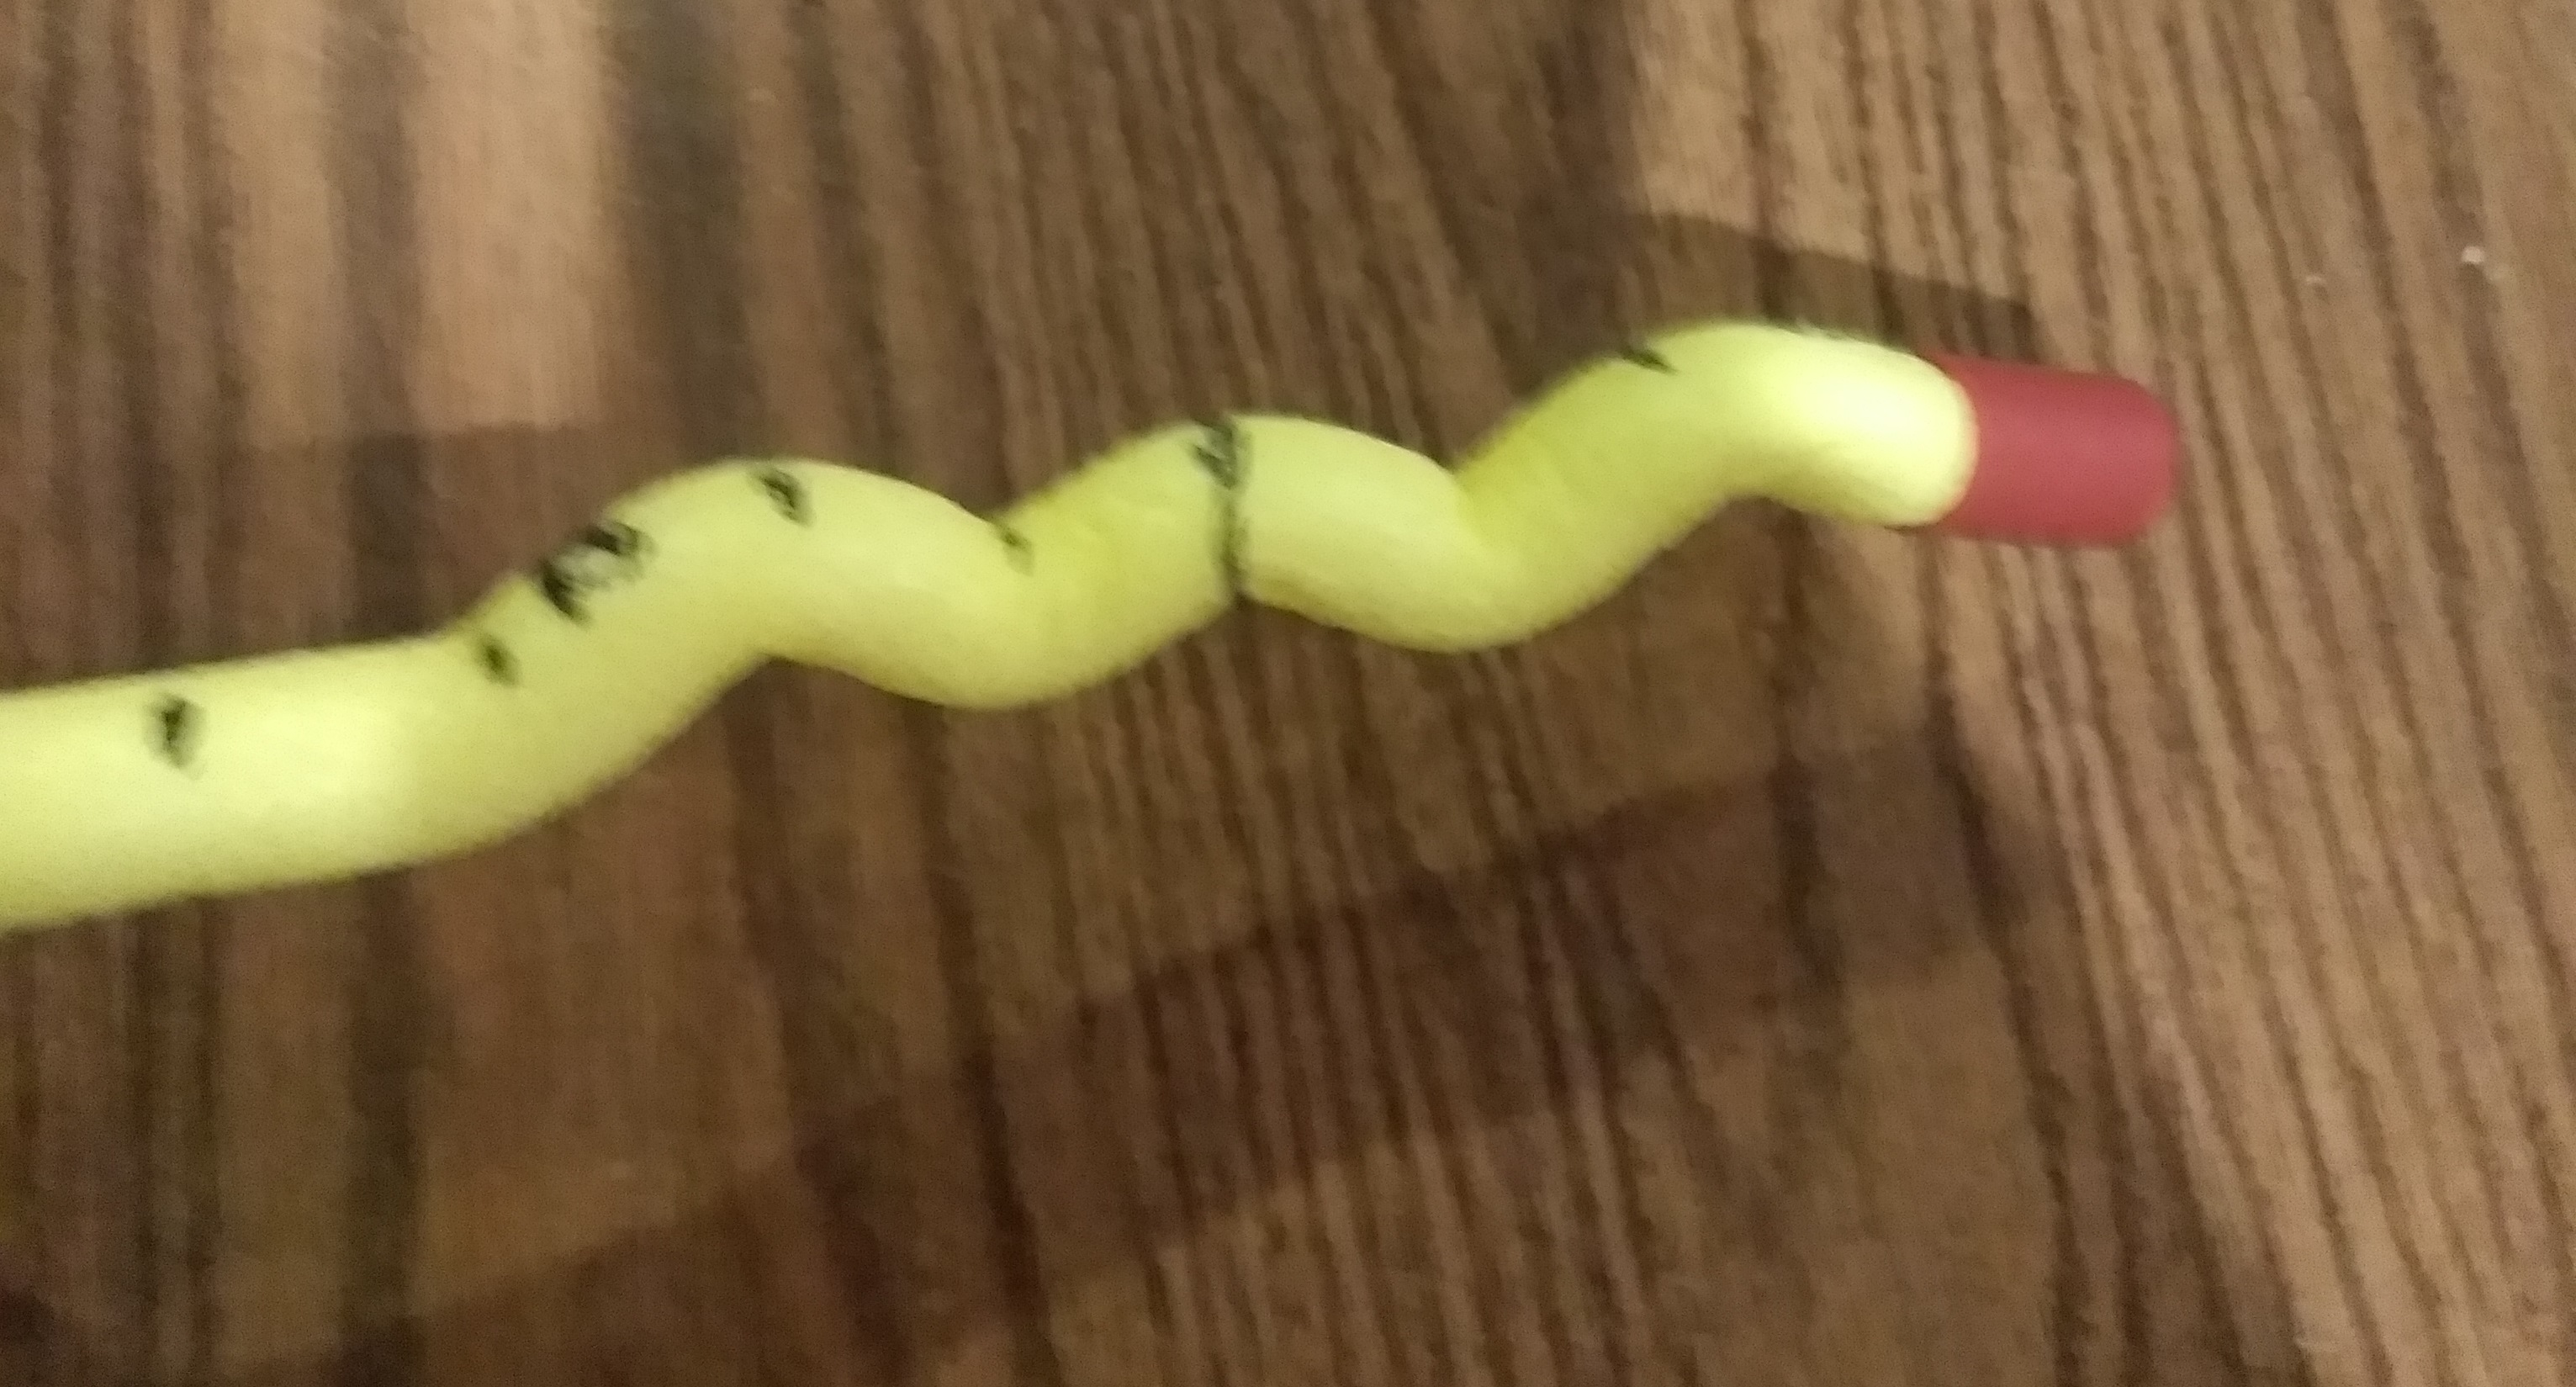
\includegraphics[scale=0.07]{sheet}
\end{figure}
Depending on the lengh of the toober, try to take around 5 minutes or less to fold secondary structures. 

After folding secondary structures, move on to tertiary structure (3D structure). Using one view on Jmol, fold the toober so you have a general shape. Next, keep changing the Jmol view, checking, and adjusting. Some good reference views are directly looking down a main helix (if it has one) (Fig. 9), and rotating it in any way. Ideally, you'd want your model to look exactly the same as the Jmol model. However, this usually doesn't happen, so try to do your best. This should take the longest, around 10-12 minutes. 
\begin{figure}[h!]
\caption{Looking directly down the alpha helix}
\centering
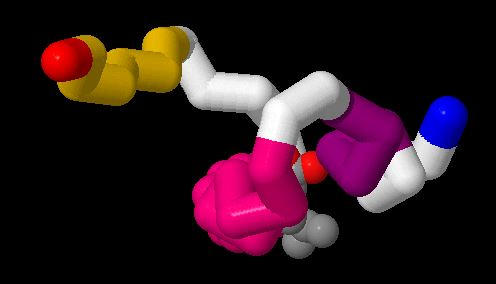
\includegraphics[scale=0.55]{direct}
\end{figure}
You should have marked the location of the sidechains on your model. Just put them on, making sure they are oriented in the right direction, and that you placed them in the correct location. You can also add support posts, wherever you feel that the structure is physically weak. You can try to shake it a little, and see which spots move around the most. Please make sure that the support posts don't mess up the structure of the protein. This final step should take around 5 minutes. Ideally, the total time to fold a protein should be around 25-30 minutes, so you can start to work on the test. Only one person should be folding the protein, and the other two should work on the test for the rest of the time. However, if you feel that you need to devote more time to the model for accuracy, you should get it as accurate as possible. 
\begin{figure}[h!]
\caption{A finished protein model}
\centering
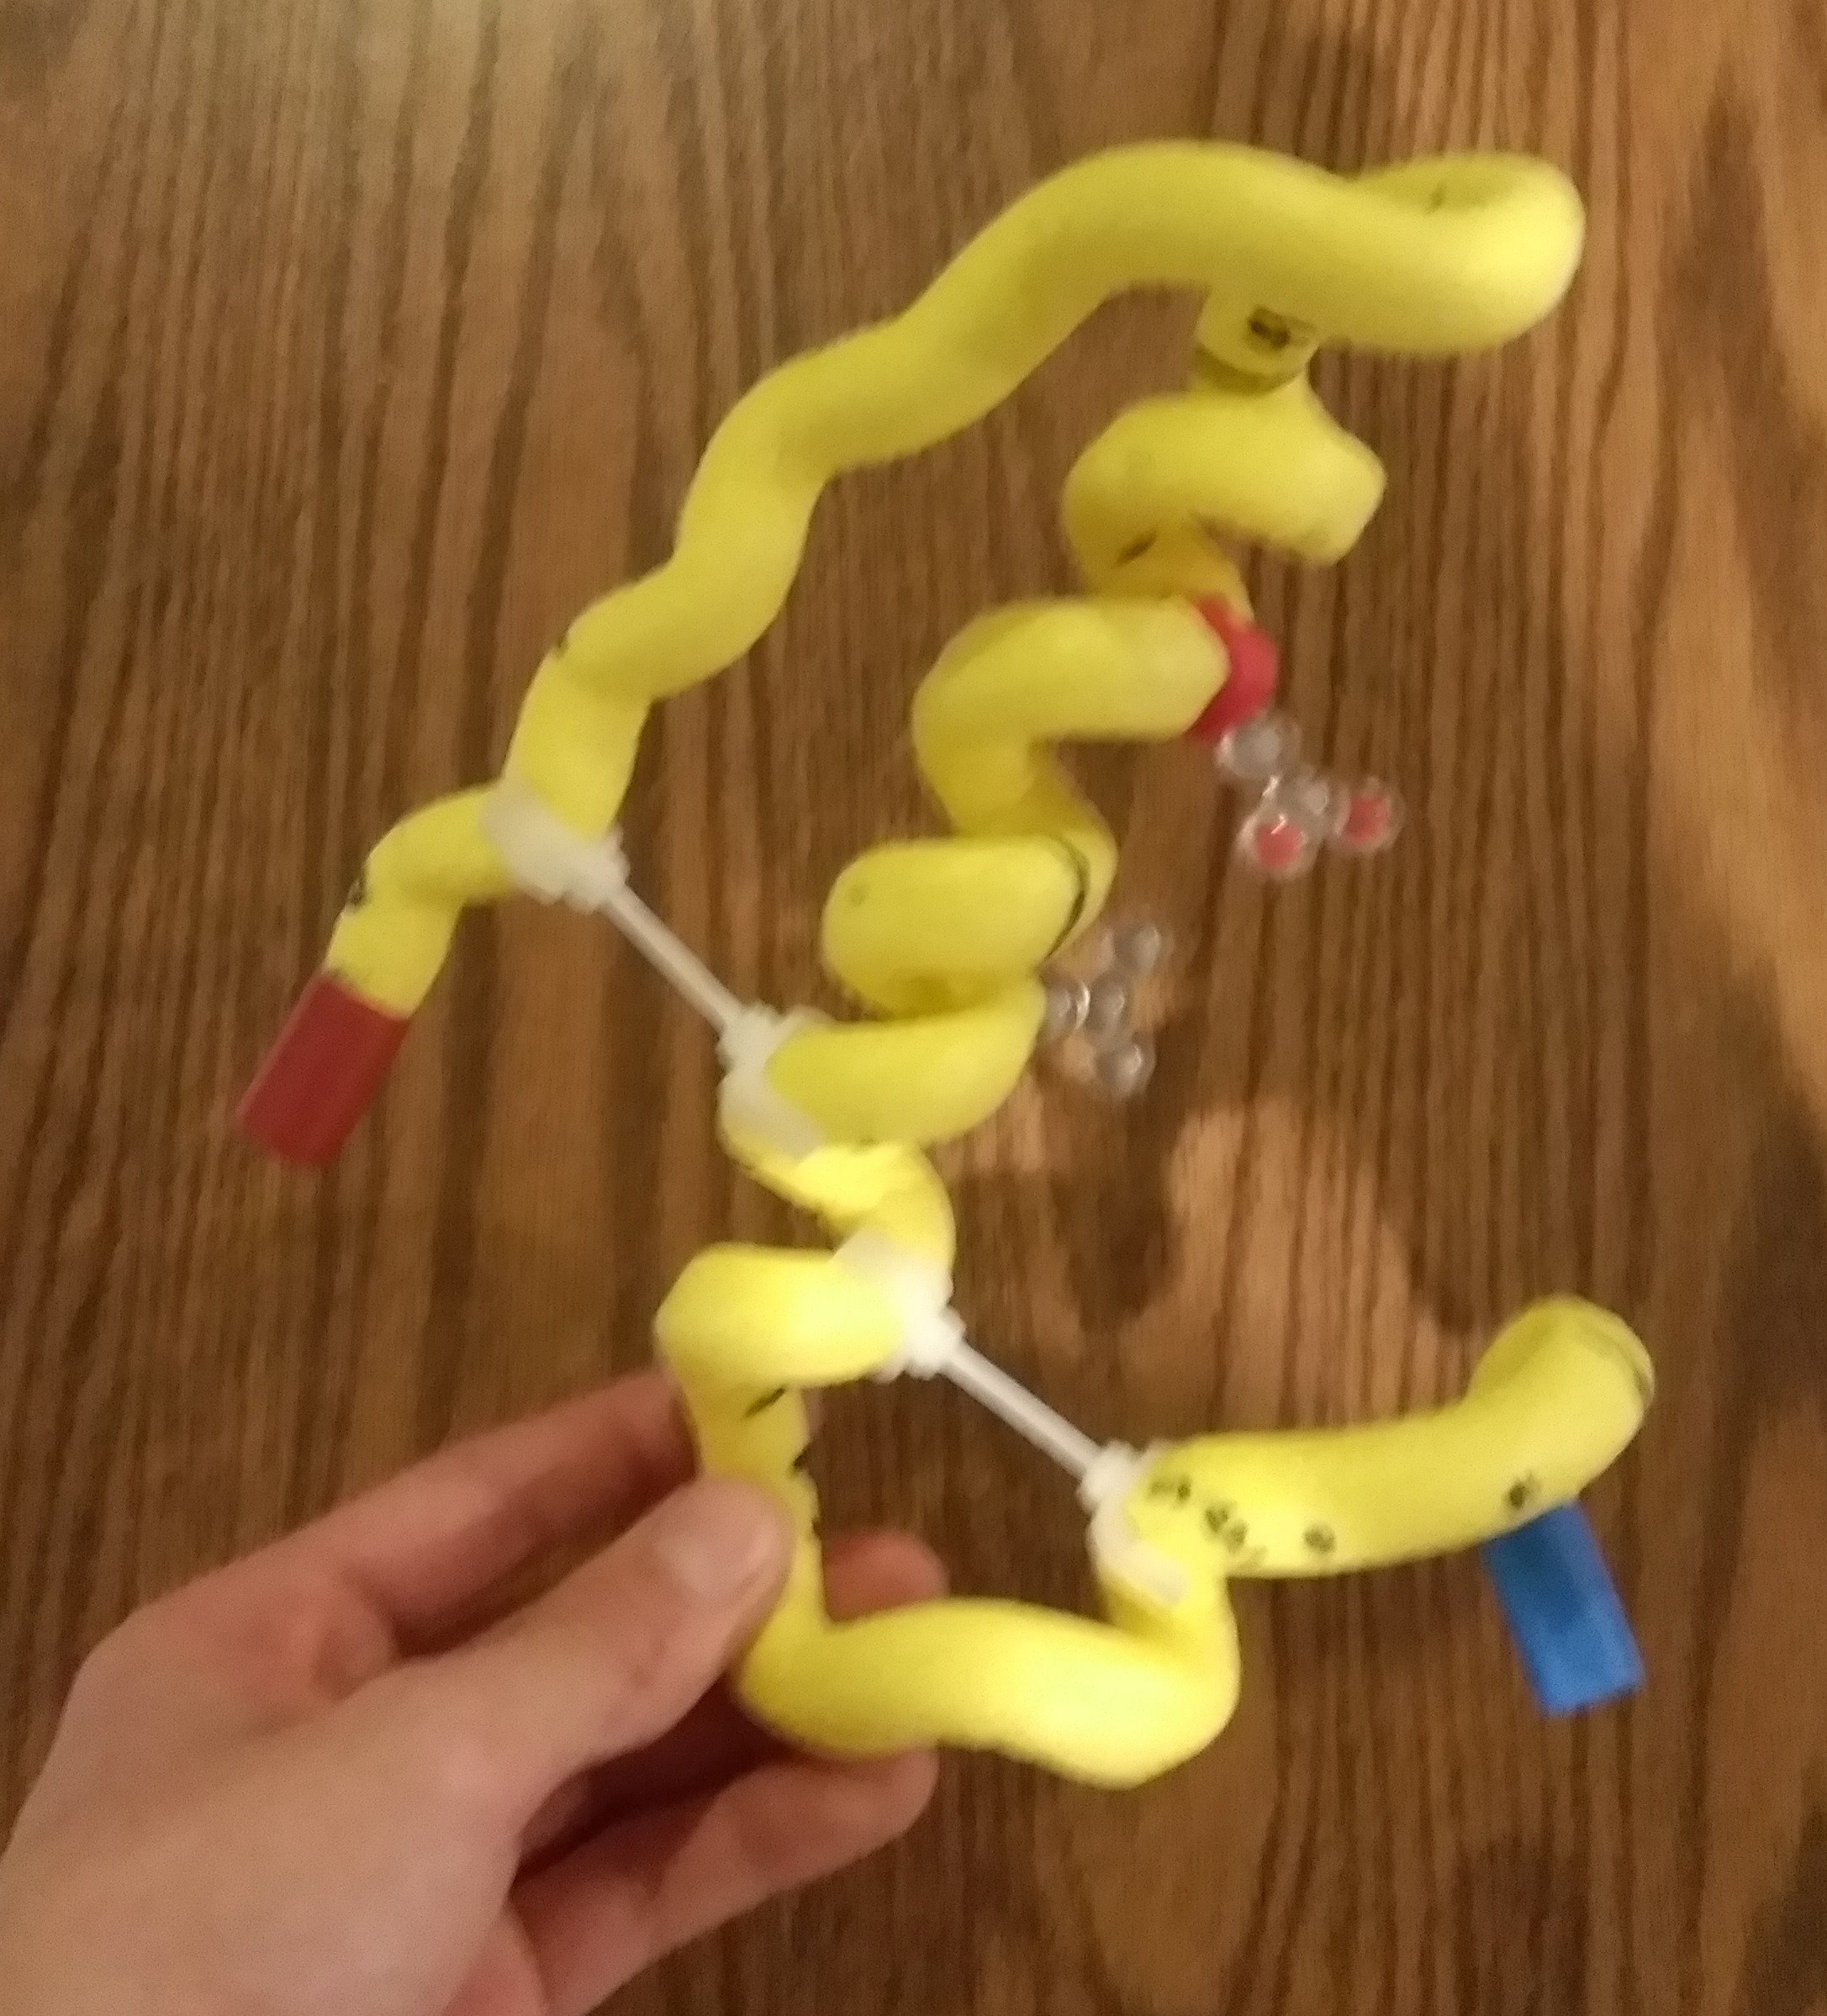
\includegraphics[scale=0.078]{finished}
\end{figure}
Here is a list of things to keep in mind: (Judges usually check for these things)
\begin{itemize}
\item The color and direction of endcaps are correct
\item The number of helices and sheets is correct
\item Helices are right handed
\item Beta sheets are folded correctly and easily recognizable
\item Secondary structures are in the correct order
\item The topology of the protein is correct (i.e. certain visually obvious `layers,' etc. 
\item The angles between various structures are correct
\item Beta strands are parallel/antiparallel, based on Jmol
\item Sidechains are in the correct location and are oriented properly. 
\end{itemize}


\section{Written Test}
The topics in the written test will mostly contain protein biochemistry, information specific to the topic, technologies in biochemistry, and some biophysics. Past cheatsheets are in the `2019' directory. 
\subsection{General Studying}
For me, I liked watching YouTube videos because it made it easier to grasp complex new topics. First, take notes in an outline form, and then, when you're ready, turn it into a cheatsheet. Look at ours as an example. 

Because of the specialized nature of this event, good and specific information can only really be obtainied from research paper. Therefore, expect to be reading a lot of these. Especially for me, these were very hard to swallow and it took me basically the whole season to really understand what they were talking about. I reccomend starting by reading those papers, even if you don't understand. After doing some research, revisit the papers and see how much more you understand. If you keep using the papers as a benchmark, you can get a lot farther and know what to learn next. The goal is to completely understand the papers, and be able to remember the main ideas without having to look at them. Indeed, many of the tests you will see are based heavily upon the papers for that year. Usually, the research papers are posted on the MSOE website. 
\subsection{Biochemistry}
You should know about amino acid properties, and how they behave within a protein. For example, in tertiary structure, hydrophobic residues tend to fold toward the center and hydrophillic residues tend to fold towards the outside. It's a good idea to include an annotated amino acid chart in your cheatsheet that contains both the properties and a picture of the structure. Know specifics on each residue, aside from the chart (This should also be a large section of your cheatsheet. )

You should also know about secondary structures, characteristics of each type, and which residues will usually be found in each type. Also know about primary structure and how it affects secondary, tertiary, and quaternary structure. 

Know about the different types of interactions within and between other proteins (van der Waal's force, disulfide bonds, hydrogen bonds, etc). Also know about denaturing proteins and applications of this. Depending on the topic for that year, you may or may not also want to know about DNA structure. 
\subsection{Techonologies in Biochemistry}
You should be farmiliar with PCR, gel electrophoresis, SEC (Size-Exclusion Chromatography), X-ray Crystallography (X-ray diffraction), Cryogenic Electron Microscopy (Cryo-EM), BLAST, and others. Usually, MSOE releases a set of research papers regarding the topic. Read the \emph{Methods} section, usually towards the end, and familiarize yourself with the listed methods. For these technologies, you should understand the principle as to why and how they work. You should also know how to interpret the data from these methods (graphs). 
\subsection{Biophysics}
This isn't a huge part of the event, but the UPenn test had a lot of it. Familiarize yourself with the thermodynamics of protein folding (Gibbs Free Energy), and know about Levinthal's Paradox and Anfinsen's dogma. 
\subsection{The Cheatsheet}
You should have a large biochem section, and a large section for the topic. Also include a section for technologies and other miscellaneous information. As previously metioned, there should be an amino acid chart. Include lots of images of the protein, and other helpful graphics. Of course, it will have to pertain to the topic, so cheatsheets will vary greatly between years. I reccomend using \LaTeX{} for cheatsheets, since it's really easy to format, but others have successfully used Google Docs and Word for cheatsheets. Of course, make sure you can read what's on the cheatsheet (Don't make the text too small). It may also be a good idea to write additional notes into the margins. Margins should be at least 0.13 in or the printer won't be able to print the stuff on the sides. 
\twocolumn[
\begin{@twocolumnfalse}
\section{Resources}
\begin{itemize}
\item MSOE CBM - http://cbm.msoe.edu/scienceOlympiad/ - very comprehensive website specifically for Protein Modeling. 
\item RCSB Protein Data Bank - http://www.rcsb.org/ - download PDB files from here. Also has links to studies relating to specific proteins. 
\item NCBI - Links to PubMed Central, BLAST, and other helpful resources. https://www.ncbi.nlm.nih.gov/
\end{itemize}
Look in the team folder for tests. I reccomend the HUSO test from 2019 and the UPenn test for Biophysics. Usually, the tests that MSOE write (Regionals and States) are more focused on the biochemistry aspect rather than the physics aspect. 

I will also put last year's research papers in the `2019' directory. 

Remember, Wikipedia and Google are your best friends! 
\end{@twocolumnfalse}
]
\end{document}